\section{Exámenes}

\subsection{Parcial 1}

\begin{problem}[1]

$\appl{d}{\real^2}{\real}$ homógenea\footnote{$(f(tx,ty) = t^mf(x,y)$} con $m>0$. F acotada superiormente sobre la circunferencia unidad.

\ppart Probar que $F$ es continua en $(0,0)$

\ppart Si $m=0$ ¿F continua en (0,0)?

\solution

\spart
\subparagraph{1)}
Vamos a ver que $F(0,0) = 0$.

$F(0,0) = F(t0,t0) = t^mF(0,0) \implies F(0,0) = 0$

\subparagraph{2)}
Aplicando la caracterización por sucesiones de la continuidad: $\{X_n\} \rightarrow 0 \implies F(X_n) \rightarrow 0$ si $F$ continua.

Sea $Z_n = \{(X_n,Y_n)\}, n\in \mathbb{N}$ una sucesión tal que $Z_n \rightarrow (0,0)$.

\begin{gather*}\abs{F_n} = \abs{F\left(\frac{Z_n}{\md{Z_n}}\md{Z_n}\right)} =
\md{X_n}^n \abs{F\left(\frac{Z_n}{\md{Z_n}}\right)} \implies \\
\exists M>0 \tlq \md{Z_n}^n \abs{F\left(\frac{Z_n}{\md{Z_n}}\right)} \leq \md{Z_n}^n M \rightarrow 0 = F(0,0)
\end{gather*}

\spart
Sí, $m=0 \implies F$ constante. Se puede demostrar pasando a coordenadas polares $x=rcos(t),y=rsen(t)$

\end{problem}

%\begin{problem}[2]
%\solution
%\end{problem}
\subsection{Enero 2013}
\begin{problem}[1]

Sea $f\in C^2(\mathbb{R})$ tal que $f(2) = 0$, $f'(2)=1$. Consideramos la ecuación \[ F(x,y,z) = x^2+y^2+z^2-f(2+Cz)=0 \]

\ppart Probar que existen un abierto $U\subset \mathbb{R}^2$ con $(0,0)\in U$, y un abierto $V\subset \mathbb{R}$ con $0\in V$, y una función $C^1$ \[ \phi: U \rightarrow V \]

tal que $F(x, y, \phi (x, y)) = 0$ para todo $(x,y) \in U$.

\ppart Hallar las derivadas parciales de la función encontrada en el apartado anterior y demostrar que

\[ y\frac{\partial  \phi (x,y)}{\partial  x} - x\frac{\partial  \phi (x,y)}{\partial  y} = 0 \]

\ppart Estudiar si la función $\phi$ alcanza un extremo relativo en $(0,0)$, y determinar su tipo (en función de la constante C).

\solution

\spart Tenemos que $F(0,0,0) = 0$, $F∈C^1$, y vemos que

\[ \frac{\partial  F}{\partial  z}(0,0,0) = 2z - Cf'(2+Cz)=-Cf'(2) = -C \neq 0 \]

con lo cual si $C \neq 0$, por el teorema de la función implícita, existen entornos $U\subset \mathbb{R}^2$ y $V\subset{R}$ con $(0,0)\in U, 0\in V$ y una función $\appl{\phi}{U}{V}$ de clase $C^1$ con $\phi (0,0) = 0$ tal que $F(x,y,\phi (x,y)) = 0 \forall (x,y)\in U$.

\spart
Derivamos implícitamente respecto de $x$:
\begin{gather*}
2\phi (x,y) \frac{\partial  \phi (x,y)}{\partial  x} - f'(2+C\phi (x,y))C\frac{\partial  \phi (x,y)}{\partial  x}=-2x \\
\hdots \\
\frac{\partial  \phi (x,y)}{\partial  x} = \frac{-2x}{2\phi (x,y) - Cf'(2+C\phi (x,y))}
\end{gather*}

 si $2\phi (x,y) \neq Cf'(2+C\phi (x,y))$.

Procediendo del mismo modo:
\[ \frac{\partial  \phi (x,y)}{\partial  y} = \frac{-2y}{2\phi (x,y) - Cf'(2+C\phi (x,y)} \]

si $2\phi (x,y) \neq Cf'(2+C\phi (x,y))$.

Multiplicando a ambos lados la derivada parcial con respecto a $x$ por $y$ y la derivada parcial con respecto a $y$ por $x$ llegamos a que \[ \frac{\partial y \phi (x,y)}{\partial  x} = x\frac{\partial  \phi (x,y)}{\partial  y} \], que era lo que queríamos demostrar.

\spart

\begin{gather*}
x^2 + y^2 + (\phi (x,y))^2 -f(2+C\phi (x,y)) = 0 \\
\frac{\partial  \phi}{\partial  x}(0,0) = \frac{0}{C} = 0 \\
\frac{\partial  \phi}{\partial  y}(0,0) = \frac{0}{C} = 0
\end{gather*}
Y por lo tanto $\phi$ tiene en $(0,0)$ un extremo relativo.

Procedemos a calcular su tipo:

\begin{gather*}
\frac{\partial  F}{\partial  x}: 2x-2\phi (x,y)\frac{\partial  \phi}{\partial  x}-f'(2+C\phi (x, y))C\frac{\partial  \phi}{\partial  x} = 0 \\
\frac{\partial  ^2 F}{\partial  x^2}(0,0): 2-2\left(\frac{\partial  \phi (x,y)}{\partial  x}\right)^2 - f''(2+C\phi (x,y))C^2\left(\frac{\partial  \phi}{\partial  x}\right)^2
\end{gather*}

Lo siento chicos... no me ha dado tiempo a copiar, es mi primer día copiando cálculo. Pero el resultado es que el extremo es:

\begin{itemize}
\item Mínimo si $C>0$
\item Máximo si $C<0$
\item Nada si $C=0$ porque $2/C$ no estaría definido.
\end{itemize}

No sé hacer matrices, pero si os apetece completar el hessiano es $(2/C, 0)$ la primera fila, y $(0, 2/C)$ la segunda fila. Por tanto el determinante da $4/C^2 > 0$ y hay que analizar el término en la fila uno, columna uno de la matriz.
\end{problem}

\begin{problem}[2] Consideramos el conjunto de todas las pirámides de base rectangular, inscritas en la esfera de radio 1, con la base paralela al plano $z=0$, y vértice en algún punto de la semiesfera interior.

\ppart Justificar que, a igualdad de base, la pirámide de mayor volumen debe tener el vértice situado en el punto $(0,0,-1)$

\ppart Hallar la longitud de las aristas que parten del vértice en la pirámide de la clase anterior que tiene volumen máximo.

\solution

\spart Planteamos la parametrización de la esfera de radio $1$

\[ Φ(θ,ρ) = \begin{pmatrix}
\cos θ \sin ρ \\
\sin θ \sin ρ \\
\cos ρ
\end{pmatrix} \]

El área de la base viene determinada por la fórmula

\[ A = \cos θ \sin θ \sin^2 ρ \]

Si fijamos este área, tenemos que, si $θ ≠ 0$

\[ \sin ρ = \sqrt{\frac{A}{\cos θ \sin θ}} = \sqrt{\frac{2A}{\sin 2θ}}\]

Por otra parte, el volumen de la pirámide será

\[ V = \frac{Ah}{3} = \frac{(\cos ρ - z_v) \cos θ \sin θ \sin^2 ρ }{3} \]

siendo $0 > z_v > -1$ el vértice de la pirámide (no ponemos un valor absoluto ya que sabemos que $z_v$ es negativo.

Veamos cuál es la base máxima de la pirámide fijado un $ρ$ dado

\[ \dpa{A}{θ} = \sin^2 ρ (\cos^2 θ - \sin^2 θ) \]

Igualando a 0, tenemos que $\cos^2 θ = \sin^2 θ$, es decir, $θ = \frac{π}{4}$. Por lo tanto, el área que tenemos que considerar es

\[ A = \frac{\sin^2 ρ}{2} \]



\end{problem}

\begin{problem}[3] Sea $S$ una superficie regular orientable y acotada en $ℝ^3$ cuyo borde es una curva cerrada regular $Γ$ de longitud $L$. Sea $\vf$ un campo $C^1$ con $\md{\vf(x,y,z)} = 2$ para todo $(x,y,z)$ tal que $\vf$ es tangente a la curva en cada punto de $Γ$.

\ppart Hallar $\int_Γ \vf \dif σ$ en función de $L$ y de la orientación de la parametrización de $Γ$.

\ppart Discutir razonadamente si puede ser $\rot \vf (x,y,z)$ para todos los puntos $(x,y,z)∈S$.

\solution

\spart Calculamos la integral, suponiendo que $Γ=σ(I)$

\[ \int_Γ \vf \dif σ = \int_I \pesc{\vf\circ σ, σ'} \dif t = \int_I \md{\vf\circ σ }\md{σ'} \dif t = 2\int_I \md{σ'} \dif t = 2 L \]

Cambiaremos de signo si la parametrización $σ$ de $L$ es negativa con respecto a $S$.

\spart Según el teorema de Stokes,

\[ \int_Γ \vf \dif σ = \iint_S \rot \vf \dif S \]

Por lo tanto, sólo podemos tener $\rot \vf = 0$ si la longitud de la curva $L=0$.

\end{problem}

\begin{problem}[4] Sea $M= \{ (x,y,z)∈ℝ^3\tq z = x^2 + y^2,\,z≤1 \}$.

\ppart Demostrar que $M$ es una variedad con borde $∂M$, determinando las dimensiones de $M$ y de $∂M$.

\ppart Supongamos $M$ con la orientación dada por un vector normal con la tercera componente negativa. Consideramos la parametrización dada por la carda $(φ,D)$ donde $φ(s,t) = (t,s,s^2+t^2)$ y $D=\{ (s,t) \tq s^2 + t^2≤ 1\}$. Estudiar si la orientación inducida por esta parametrización coincide o no con la definida inicialmente.

\ppart Determinar la orientación compatible o inducida en la frontera $∂M$.

\ppart Calcular

\[ \iint_M \rot \vf \dif S \]

siendo $\vf(x,y,z) = (x,y,e^{-(x^2+y^2)})$.

\solution

\spart Nos están dando una parametrización (la del apartado \textbf{b)}), así que si demostramos que es una paramterización habremos demostrado que es una subvariedad. Obviamente, $φ∈C^\infty$ y su inversa es continua ($\inv{φ}(x,y,z) = (x,y)$) y $C^1$. Además, el rango de su diferencial es máximo siempre. Como $\appl{φ}{ℝ^2}{ℝ^3}$, $M$ es una subvariedad de dimensión 2. La frontera son los puntos que cumplen $z=1$ (o $s^2 +t^2=1$), y es de dimensión 1.

\spart Calculamos el vector tangente según la parametrización:

\[ \begin{matrix}
 \\ φ_s= \\ φ_t=
\end{matrix}
\left|
\begin{matrix}
\vec{i}	& \vec{j} & \vec{k} \\
0		& 1		  & 2s		\\
1		& 0 	  & 2t
\end{matrix}
\right|
= \begin{pmatrix}
2t \\ 2s \\ -1
\end{pmatrix}
\]

La tercera coordenada es negativa y por lo tanto la orientación coincide.

\spart Parametrizamos $∂M$ por la aplicación

\begin{align*}
\appl{σ&}{[0,2π]}{ℝ^3} \\
σ(θ) &= (\cos θ , \sin θ, 1)
\end{align*}

Su vector tangente es $σ'(θ) =(-\sin θ , \cos θ, 0)$, que tiene la orientación que quiera tener.

\spart

Según el teorema de Stokes, \[ \iint_M \rot \vf \dif S = \int_{∂M} \vf \dif σ \]

Calculamos:

\begin{align*}
\int_{∂M} \vf \dif σ &= \int_0^{2π} \pesc{\vf \circ σ, σ'} \dif θ = \int_0^{2π} \pesc{(\cos θ, \sin θ, e^{-1}),(-\sin θ , \cos θ, 0)} \dif θ = \\
&= \int_0^{2π}-\sin θ \cos θ + \sin θ \cos θ \dif θ = \\
&= 0
\end{align*}

\end{problem}

\subsection{Junio 2013}

\begin{problem}[1]
 Sea $\appl{f}{\mathbb{R}^3}{\mathbb{R}}$. Se dice que f es homogénea de grado m si
\[ f(\lambda x, \lambda y, \lambda z) = \lambda ^m f(x,y,z) \] para todo $\lambda > 0$.

\ppart  Si f es diferenciable y homogénea de grado $m>0$ demostrar que:
\[ \pesc{\nabla f(x,y,z), (x,y,z)} = mf(x,y,z) \]

\ppart Supongamos $f$ continua sobre la esfera ${x^2+y^2+z^2=1}$. Supongamos que $f$ es homogénea de grado $m = 0$, y que $f(0,0,0) = 0$.

\begin{itemize}
\item Estudiar la continuidad de $f$ en el origen.
\item Estudiar la continuidad de $f$ en el resto de puntos del espacio.
\end{itemize}

\solution

\spart \[ x\frac{\partial  f}{\partial  x}(x,y,z) + y\frac{\partial  f}{\partial  y}(x,y,z) + z\frac{\partial  f}{\partial  z}\]
derivamos respecto de $\lambda$

$$\frac{\partial  f}{\partial  \lambda}(\lambda x, \lambda y, \lambda z) = \underbrace{\frac{\partial }{\partial  \lambda}(\lambda^mf(x,y,z))}_{m\lambda^{m-1}f(x,y,z)}$$

$$\frac{\partial  f}{\partial  \lambda x}\frac{\partial  \lambda x}{\partial  \lambda} + \frac{\partial  f}{\partial  \lambda y}\frac{\partial  \lambda y}{\partial  \lambda} + \frac{\partial  f}{\partial  \lambda z}\frac{\partial  \lambda z}{\partial  \lambda} = \frac{\partial  f}{\partial  \lambda x}x + \frac{\partial  f}{\partial  \lambda y}y + \frac{\partial  f}{\partial  \lambda z}z = m\lambda ^{m-1} f(x,y,z) $$

$$\pesc{\nabla f(\lambda x,\lambda y,\lambda z), (x,y,z)} = m\lambda^{m-1} f(x,y,z)\ \forall \lambda > 0$$

Si tomamos $\lambda = 1$ entonces $$\pesc{\nabla f(x,y,z), (x,y,z)} = mf(x,y,z)$$ que era lo que queríamos demostrar.\footnote{Este es el teorema de Euler de las funciones homogéneas, y sí, te piden demostrarlo en un examen, extraordinario}


\spart
Considero\footnote{Esto es una idea feliz.} $\lambda = \frac{1}{\norm{(x,y,z)}}$\\
\[ f(x,y,z) = f(\lambda x, \lambda y, \lambda z) \]
Si f es continua en $x_1$ lo va a ser en $x_2$ con $x_1 = \lambda x_2$ por se homogénea.\footnote{Es como tomar un punto $x_2$ en una esfera más pequeña de la esfera de radio uno, y si unimos ese punto con el $x_1$ que esta en la esfera de radio uno, por ser homogénea va a ser continua en la recta que los une.}

Formalmente:

\begin{gather*}
\forall \epsilon > 0, \exists δ  > 0 \tq  \norm{x-y} < δ  \implies \norm{f(x) - f(y)} < \epsilon \\
\norm{x - 0} < δ  \implies \abs{f(x,y,z) - f(0,0,0)} < \epsilon \\
\abs{f(x,y,z)} < \epsilon\ \forall \epsilon > 0 \\
 f = 0 \\
 \frac{x}{\norm{x}} - \frac{y}{\norm{y}} < \norm{x-y}
 \end{gather*}

\end{problem}

\begin{problem}[2] Sea $A=\{\frac{1}{4}≤ x^2 + y^2 ≤ 1\}$. Consideramos $\appl{F}{A}{ℝ^2}$,

\[ (x,y)\mapsto F(x,y) = \left(\frac{x}{x^2+y^2},\frac{y}{x^2+y^2}\right) \]

\ppart Determinar la imagen del conjunto $A$, $F(A)$.

\ppart Estudiar si $F$ es localmente invertible, con inversa diferenciable.

\ppart Estudiar si existe una inversa global, definida sobre todo el conjunto $F(A)$.

\solution

\spart \[ F(A) = \{ (x,y) \tq 4 ≥ x^2 + y^2 ≥ 1 \} \]

\spart Calculamos el diferencial:

\[ DF(x,y) = \begin{pmatrix}
\frac{x^2+y^2 - 2x^2}{(x^2+y^2)^2} & \frac{-2yx}{(x^2+y^2)^2} \\
\frac{-2xy}{(x^2+y^2)^2} & \frac{x^2+y^2 - 2y^2}{(x^2+y^2)^2}\\
\end{pmatrix} = \frac{1}{(x^2+y^2)^2}\begin{pmatrix}
x^2+y^2 - 2x^2 & -2yx \\
-2xy & x^2 + y^2 - 2y^2 
\end{pmatrix} \]

y su determinante es  (ignorando el factor que no se anula)

\begin{align*}
 \det DF(x,y) &= ((x^2+y^2) - 2x^2)((x^2+y^2)-2y^2) -2x^2y^2 = \\
 	&= (x^2+y^2)^2 -2(x^2+y^2)^2 + 2x^2y^2 - 2x^2y^2 = \\
 	&= -(x^2+y^2)^2 
\end{align*}

que es distinto de 0 en $A$. Por lo tanto, aplicamos T.F.Inversa y listos.

\spart La función existe porque $F$ es biyectiva sobre su imagen. Y no me apetece probarlo, pero se ve.

\end{problem}

\begin{problem}[3]

\ppart Consideramos la familia de curvas dependiente de parámetro $k$, $M_k=\{ z= x^2-y^2 \} \cap \{ z= k \}$. Determinar para qué valores de $K$ el conjunto $M_k$ es una variedad de dimensión 1 en $ℝ^3$.

\ppart Sea $M=\{x^2+y^2+z^2=4\} \cap \{x^2+(y-1)^2=1\}$. Demostrar que la parte de $M$ contenida en el interior del semiespacio superior $z>0$ es una variedad $C^1$ y determinar su dimensión. Demostrar que globalmente $M$ no es una variedad en $ℝ^3$

\solution

\spart Nos dan $M$ como un sistema de ecuaciones $F=0$, con $\appl{F}{ℝ^3}{ℝ^2}$. Tenemos que ver si su diferencial tiene rango máximo cuando $F=0$.

\[ DF = \begin{pmatrix}
2x & 2y & 1 \\
0 & 0 & 1
\end{pmatrix} \]

Si $k≠0$, o bien $x$ o bien $y$ son distintos de 0 (si no no se cumpliría $x^2-y^2 = k$) y $DF$ tiene rango máximo. Por lo tanto, $M_k$ es variedad 1-dimensional si $k≠0$.

\spart

\end{problem}

\begin{problem}[4] Sea $S$ la superficie cerrada limitada por la semiesfera $z= \sqrt{9-x^2-y^2}$ y la parte superior del hiperboloide $x^2+y^2-z^2=-1$ con la orientación inducida por la normal exterior. Consideramos el campo

\[ \vf = (xz+\cos y \sin z,yz+e^{xz},z^2+e^y) \]

Calcular el flujo $\iint_S\vf \dif S$.

\solution El amigo Gauss nos dice que

\[ \iint_S \vf \dif S = \iiint_{Ω} \dv \vf \id{x,y,z} \]

Así que vamos a ver qué nos da la divergencia.

\[ \dv \vf = z + z + 2z = 3z \]

\begin{wrapfigure}{r}{0.5\textwidth}
  \begin{center}
    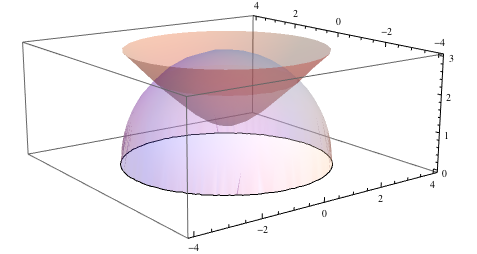
\includegraphics[width=0.48\textwidth]{imgs/ExamenJunio_Ej4.png}
  \end{center}
  \caption{El coso a integrar.}
\end{wrapfigure}


Sale algo simple (menos mal) así que podemos tratar de parametrizar $Ω$. La dividimos en dos partes: una, la limitada por el hiperboloide, y otra, la limitada por la semiesfera. Para que todo sea menos feo, hacemos un cambio a coordenadas cilíndricas, cuyo cambio en la medida es $r$:

\begin{multline*}
\iiint_Ω \dv \vf \id{x,y,z} = \\ \iiint_Ω 3z \cdot r \id{z,θ,r} = I_E + I_H
\end{multline*}

Calculamos la intersección del hiperboloide y la esfera:

\[ r^2 - 9 + r^2 = -1 \implies 2r^2 = 8 \implies r = 2 \]

Entonces la integral de la esfera nos queda

\begin{align*}
 I_E &= \int_2^3\int_0^{2π}\int_0^{\sqrt{3-r^2}} 3zr \id{z,θ,r} = \\
 	&= 3\int_2^3r\int_0^{2π}\eval{\frac{z^2}{2}}_{z=0}^{\sqrt{3-r^2}} \id{θ,r} = \\
 	&= \frac{3}{2} \int_2^3 r \int_0^{2π} 3-r^2 \id{θ,r} = \\
 	&= \frac{2π3}{2} \int_2^3 3r - r^3 \dif r = \\
 	& \dots
\end{align*}

Y de la misma forma

\begin{align*}
I_H &= \int_0^2\int_0^{2π}\int_0^{\sqrt{r^2+1}} 3zr \id{z,θ,r} = \\
	&= \dots
\end{align*}

La resolución de la integral se deja como ejercicio para el lector que a mí ya me da pereza.

\end{problem}